\documentclass[aspectratio=169]{beamer}
\usetheme[block=fill]{metropolis}
\usepackage{tikz}
\usetikzlibrary{shapes.geometric, arrows.meta, positioning, calc}

\title{Building a Reproducible Scholarly Search Toolkit}
\subtitle{Episode 21: GitHub Actions \& CI/CD}
\author{Scholar Search Kit}
\date{}

\begin{document}

\begin{frame}[plain]
  \titlepage
\end{frame}

\begin{frame}{Episode Goal}
  \begin{alertblock}{The Goal}
    Set up Continuous Integration (CI) to automatically run tests and linters every time code is pushed to GitHub.
  \end{alertblock}
  \vspace{0.5cm}
  If an open-source contributor opens a Pull Request, you cannot blindly trust it. We need a robot to verify that their code doesn't break our tests.
\end{frame}

\begin{frame}{The CI Workflow}
  \begin{center}
  \resizebox{0.7\linewidth}{!}{
  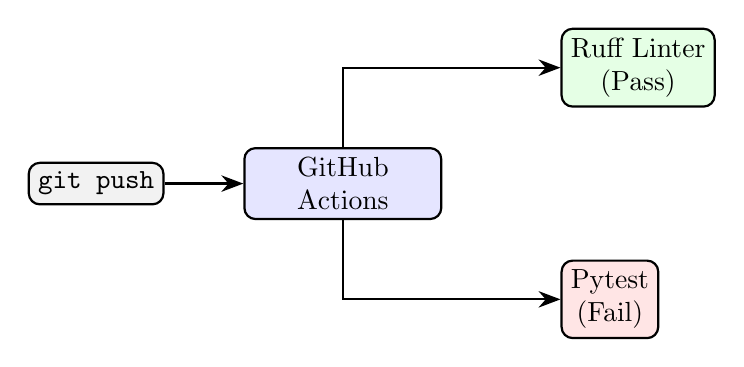
\begin{tikzpicture}[
      node distance=1.5cm and 1cm,
      dev/.style={rectangle, draw, thick, rounded corners, fill=black!5, align=center},
      gh/.style={rectangle, draw, thick, rounded corners, minimum width=2.5cm, fill=blue!10, align=center},
      job/.style={rectangle, draw, thick, rounded corners, fill=green!10, align=center},
      fail/.style={rectangle, draw, thick, rounded corners, fill=red!10, align=center},
      arrow/.style={-{Stealth[scale=1.2]}, thick}
    ]
    
    \node[dev] (push) {\texttt{git push}};
    \node[gh, right=of push] (action) {GitHub\\Actions};
    \node[job, above right=0.5cm and 1.5cm of action] (lint) {Ruff Linter\\(Pass)};
    \node[fail, below right=0.5cm and 1.5cm of action] (test) {Pytest\\(Fail)};
    
    \draw[arrow] (push) -- (action);
    \draw[arrow] (action) |- (lint);
    \draw[arrow] (action) |- (test);
  \end{tikzpicture}
  }
  \end{center}
  \vspace{0.2cm}
  A YAML file tells GitHub to spin up a virtual Ubuntu server, install Python, and run our checks.
\end{frame}

\begin{frame}{Implementation: Testing Multiple Versions}
  \begin{block}{The Matrix}
    Researchers use different versions of Python (3.10, 3.11, 3.12).
  \end{block}
  
  \begin{itemize}
      \item We use a GitHub Actions \textit{Matrix Strategy}.
      \item The workflow automatically runs the test suite 3 times simultaneously, once for each Python version.
      \item This guarantees our code is backwards compatible.
  \end{itemize}
\end{frame}

\begin{frame}{Verification}
  \begin{alertblock}{Success Criteria}
    \begin{itemize}
        \item A \texttt{.github/workflows/ci.yml} file is created.
        \item Pushing a deliberate syntax error causes the GitHub Action to fail and block the Pull Request.
    \end{itemize}
  \end{alertblock}
\end{frame}

\end{document}
